\documentclass{scrbook}
\usepackage{graphicx} % Required for inserting images
\usepackage{tabularx} % Required for fixed width tables
\usepackage{scrlayer-scrpage} % Required for the subtitles
\usepackage{url} % Required for the URLs
\usepackage{hyperref} % Required for the URLs
\usepackage{listings} % Required for the code snippets

% Put the caption of the snippets at the bottom
\lstset{
    captionpos=b
}


\title{eXtensible Markup Language}
\subtitle{Ambient intelligence course (A.Y. 2025/2026)\\Topic taught by Prof. Floriano Scioscia}
\author{Gabriele Colapinto}
\date{\today}

\begin{document}

\maketitle
\thispagestyle{empty}

{\Large\textbf{License}} \\
{Notes from Ambient intelligence (A.Y. 2025/2026) by Gabriele Colapinto. 
Course taught by professors Michele Ruta, Floriano Scioscia, Arnaldo Tomasino, Davide Loconte — 
Licensed under CC BY-NC 4.0.\\
\url{https://creativecommons.org/licenses/by-nc/4.0/}}

\vspace*{\fill}
\rule{\textwidth}{0.2pt}
\small{© 2025 Gabriele Colapinto \\
Released under the \href{https://creativecommons.org/licenses/by-nc/4.0/}{Creative Commons Attribution–NonCommercial 4.0 International License}}

\clearpage

\tableofcontents

\chapter{Core Concepts of XML}

\section{Defining XML: Purpose and Design Goals}

The Extensible Markup Language (XML) is a foundational technology designed to store, transport, and interchange data in a format that is both human-readable and machine-readable. Its strategic importance lies in its ability to provide a standardized, platform-independent syntax for describing information, making it an essential tool for data exchange between disparate systems and across the web. At its core, XML is a meta-language; it does not have predefined tags but instead provides a framework for authors to define their own markup languages tailored to specific applications. \\

XML's architecture was predicated on a clear set of design goals intended to maximize its utility, interoperability, and ease of use. These goals, established by the World Wide Web Consortium (W3C), are as follows:

\begin{itemize}
    \item
    \textbf{Straightforward usability over the Internet:} XML is a text-based format designed to be easily transmitted and processed over standard internet protocols.

    \item
    \textbf{Support for a wide variety of applications (extensibility):} Authors can create custom tags to describe any kind of structured or semi-structured data, making it adaptable to countless domains.

    \item 
    \textbf{Ease of document creation:} The rules for creating XML documents were designed to be simple enough for both humans and automated tools to generate them easily.

    \item 
    \textbf{Simplicity for writing processing programs:} The language's strict and predictable syntax simplifies the development of software that parses, validates, and manipulates XML documents.

    \item 
    \textbf{Human-legibility:} XML documents are reasonably clear and can be read and understood by people without specialized tools.
\end{itemize}

These principles have enabled XML to serve as a robust foundation for countless data formats and protocols. To fully appreciate its design, it is useful to understand the historical context from which it emerged.

\section{Historical Context and Relationship to SGML and HTML}

Understanding XML’s origins is key to grasping its design choices and its relationship with other critical web languages like SGML and HTML. The language was not created in a vacuum but as a direct evolution of preceding markup standards, refined specifically for the challenges of the modern web.\\

XML is a simplified subset of the \textbf{Standard Generalized Markup Language (SGML)}, a powerful but complex international standard for defining markup languages that was established in 1986. SGML is also the parent language of HTML (HyperText Markup Language). While both XML and HTML share this common ancestor, they were designed for different purposes and with different philosophies. HTML was developed with a relaxed syntax, allowing web browsers to make a best-effort attempt to render pages even if they contained errors. In contrast, XML adopted a much stricter syntax, a deliberate choice to ensure reliability and predictability when processing both semi-structured documents and highly structured data, such as that exported from a database. This rigidity makes XML documents unambiguous and easier for applications to parse correctly. \\

The evolution of XML and its related standards can be summarized by a few key milestones:

\begin{itemize}
    \item 
    \textbf{1997:} The first XML Working Draft was released by the W3C.

    \item 
    \textbf{1998:} XML 1.0 was published as a formal W3C Recommendation.

    \item 
    \textbf{ 2006:} XML 1.1 was released as a W3C Recommendation, coexisting with version 1.0.
    
\end{itemize}

Having established what XML is and where it came from, we can now examine how its structure facilitates the organization of complex information.

\chapter{The Structure of an XML Document}

\section{The XML Tree and Core Components}

\begin{figure}
  \centering
  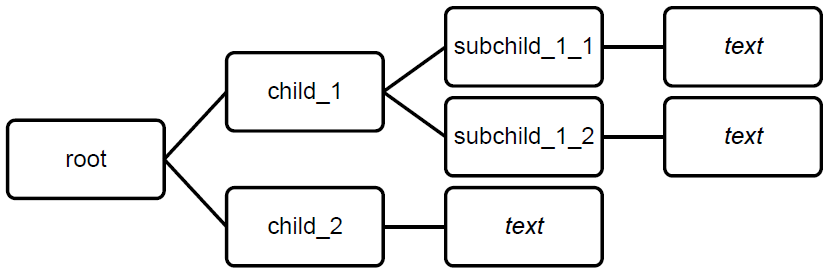
\includegraphics[width=\textwidth]{Images/XML_tree.png}
  \caption{XML tree}
\end{figure}

All XML documents are fundamentally structured as a logical tree, a hierarchical model that is crucial for parsing and data retrieval. This hierarchical model is not arbitrary; it maps directly to the nested structures common in both documents and data records, making it a natural and computationally efficient paradigm for parsers. The tree begins with a single "root" element and branches out to "child" elements, which can in turn have their own children (sub-elements), allowing for the representation of complex, multi-level data relationships. \\

The primary components for building this tree are \textbf{elements} and \textbf{attributes}. An element is a structural block, defined by a start tag and an end tag, that can contain text, other elements, or a mix of both. An attribute is a name-value pair located inside an element's start tag, designed to hold simple, atomic data that describes the element itself. The choice between using an element or an attribute depends on the nature of the data. As a general rule, elements are preferred for complex, structured, or potentially expandable data, while attributes are best suited for simple metadata. \\

Table 2.1 contains two examples of comparison of usage of elements and attributes while table 2.2 contains the comparison of their key characteristics. In both examples we use a note and a person to illustrate the concepts.

\begin{table}[h!]
    \centering
    \begin{tabularx}{\textwidth}{|X|X|X|}
        \hline
        \textbf{Example} & \textbf{Elements version} & \textbf{Attributes version} \\
        \hline

        \textbf{note} & Listing~\ref{lst:note_elements} & Listing~\ref{lst:note_attributes} \\
        \hline

        \textbf{person} & Listing~\ref{lst:person_elements} & Listing~\ref{lst:person_attributes} \\
        \hline
    \end{tabularx}
    \caption{Comparison of usage of elements and attributes}
\end{table}

\begin{lstlisting}[language=XML, caption={note with elements}, label={lst:note_elements}]
<note>
    <day>10</day>
    <month>01</month>
    <year>2008</year>
    <to>Tove</to>
    <from>Jani</from>
    <heading>Reminder</heading>
    <body>Don't forget me this weekend!</body>
</note>
\end{lstlisting}

\begin{lstlisting}[language=XML, caption={note with attributes}, label={lst:note_attributes}]
<note
    day="10"
    month="01"
    year="2008"
    to="Tove"
    from="Jani"
    heading="Reminder"
    body="Don't forget me this weekend!">
</note>
\end{lstlisting}

\begin{lstlisting}[language=XML, caption={person with elements}, label={lst:person_elements}]
<person>
    <gender>female</gender>
    <name>Jane</name>
    <surname>Doe</surname>
    <date_of_birth>01/01/1990</date_of_birth>
</person>
\end{lstlisting}

\begin{lstlisting}[language=XML, caption={person with attributes}, label={lst:person_attributes}]
<person
    gender="female"
    name="Jane"
    surname="Doe"
    date_of_birth="01/01/1990">
</person>
\end{lstlisting}

\begin{table}
    \centering
    \begin{tabularx}{\textwidth}{|X|X|X|} \hline
        Feature & Elements & Attributes \\ \hline

        \textbf{Content} &
        Can contain text, other elements, or a mix. For example, \texttt{\textless note\textgreater} contains child elements like \texttt{\textless to\textgreater} and \texttt{\textless body\textgreater}. &
        Designed to contain data related to a specific element; cannot contain tree structures. For example, \texttt{\textless person gender="female"\textgreater}. \\ \hline

        \textbf{Values} &
        Can have complex, nested content. &
        Cannot contain multiple values. \\ \hline

        \textbf{Expandability} &
        Easily expandable for future changes. New child elements can be added without breaking existing structure. &
        Not easily expandable. Adding new attributes can be more disruptive to processing logic. \\ \hline

    \end{tabularx}
    \caption{Comparison of elements and attributes}
\end{table}

For any software to process this tree structure, the document must first adhere to a fundamental set of syntax rules. A document that meets these criteria is known as being "well-formed."

\section{Rules for Well-Formed XML}

The concept of a "well-formed" XML document is non-negotiable. Before any XML parser can read or validate a document, it must first confirm that the document is syntactically correct. If a document is malformed, a compliant application is required to stop processing and report an error. This strictness ensures data integrity and prevents the ambiguity that can arise from inconsistent parsing of flawed documents. \\

The essential syntax rules for creating a well-formed XML document are as follows:

\begin{enumerate}
    \item
    \textbf{Optional Prolog:} The XML prolog, which declares the XML version and character encoding, is optional. If it exists, it must be the very first line of the document.

    \item
    \textbf{Single Root Element:}  Every document must have exactly one root element that contains all other elements.

    \item
    \textbf{Required Closing Tags:} All elements must have a closing tag. Elements without content, known as empty elements, can use a self-closing tag format.

    \item
    \textbf{Case Sensitivity:} Tags are case-sensitive. The start tag and end tag must match exactly.

    \item 
    \textbf{Proper Nesting:} Elements must be nested correctly without overlapping. An element opened inside another must be closed before the outer element is closed.

    \item 
    \textbf{Quoted Attributes:} Attribute values must always be enclosed in single or double quotes.

    \item 
    \textbf{Entity References:} Special characters that are part of the XML syntax itself (like \textless and \&) must be represented using entity references to avoid being misinterpreted by the parser.
\end{enumerate}

Once a document is confirmed to be well-formed, the next challenge is ensuring it can be correctly interpreted across different systems, which requires addressing potential ambiguities at both the character and element levels.

\begin{figure}
  \centering
  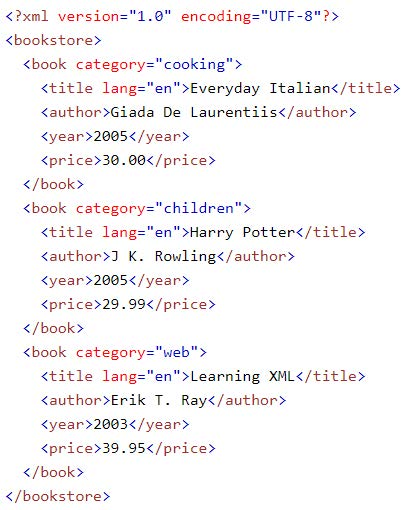
\includegraphics[width=\textwidth]{Images/XML_example.jpg}
  \caption{Example of XML well formed document}
\end{figure}

\chapter{Achieving Interoperability}

\section{Character Encoding}

When XML was created in the 1990s, one of the most significant challenges to data interchange was the lack of a universal character encoding standard. Different platforms, vendors, and industries adopted widely different encodings, creating a situation where a text file created on one system could be unreadable on another. Exchanging a document "over the wire" meant sending a stream of ones and zeros, and without a shared understanding of how to interpret that stream, data was easily corrupted. \\ 

XML's solution to this chaotic landscape was both simple and elegant: a declarative approach. The optional \texttt{encoding} attribute in the XML prolog (e.g., \texttt{\textless ?xml version="1.0" encoding="UTF-8"?\textgreater}) explicitly tells the processing application which character encoding was used to create the document. This declaration allows the receiving system to interpret the stream of characters correctly, regardless of its own default settings. \\ 

This design was forward-thinking, providing a mechanism to support both modern standards like Unicode (e.g., UTF-8) and legacy encodings required by older systems. While character encoding solves ambiguity in the interpretation of text, another mechanism—namespaces—is required to solve ambiguity in the meaning of element names.

\section{Namespaces}

As XML usage grew, a new problem emerged: name collisions. When mixing or combining XML documents from different applications, it is common for elements to have the same name (e.g., \texttt{\textless course\textgreater}) but entirely different meanings, content, or structures. Without a way to distinguish between them, a processing application would be unable to interpret the data correctly. \\

For example, consider two different XML applications that both use a \texttt{\textless course\textgreater} element. One might describe academic courses, while the other describes meal courses: \\

\begin{lstlisting}[language=XML, caption=Example of ambiguous applications]
    <!-- From an academic application -->
    <courses>
      <course cfu="9">Information Systems</course>
      <course cfu="12">Operating Systems</course>
    </courses>
    
    <!-- From a culinary application -->
    <courses>
      <course>First Course: Soup</course>
      <course>Main Course: Steak</course>
    </courses>
\end{lstlisting}

XML Namespaces solve this problem by allowing authors to qualify element names with a prefix. This is achieved using a special attribute, \texttt{xmlns:prefix="URI"}, which associates a short prefix (e.g., \texttt{lif}) with a unique Uniform Resource Identifier (URI). The URI acts as a universal, unambiguous identifier for the vocabulary. The combination of the prefix and the element name creates a "qualified name" that resolves the collision. \\

Once a document is well-formed and its terms are made unambiguous through namespaces, it can be further strengthened by validating it against a formal set of structural rules known as a schema.

\chapter{Validating XML with Schemas}

\section{Introduction to Validation: DTD and XSD}

There is a critical distinction between a "well-formed" XML document and a "valid" one. A well-formed document adheres to all the basic syntax rules of XML, making it parsable. However, this says nothing about whether its structure is appropriate for a particular application. Validation is the process of checking a well-formed document against a \textbf{schema}—a formal contract that defines the required structure, element names, data types, and constraints for a specific class of documents. A document that passes this check is considered "valid." Validation is essential in business-to-business data exchange, where the schema acts as a formal, enforceable contract between parties. \\

The two primary schema languages for XML are \textbf{Document Type Definition (DTD)} and \textbf{XML Schema Definition Language (XSD)}. DTD is the original schema language, inherited from SGML, and is relatively simple. XSD is a more powerful, flexible, and feature-rich successor that is itself written in XML. We will begin by exploring the capabilities and limitations of DTD.

\section{Document Type Definition (DTD)}

\begin{figure}
  \centering
  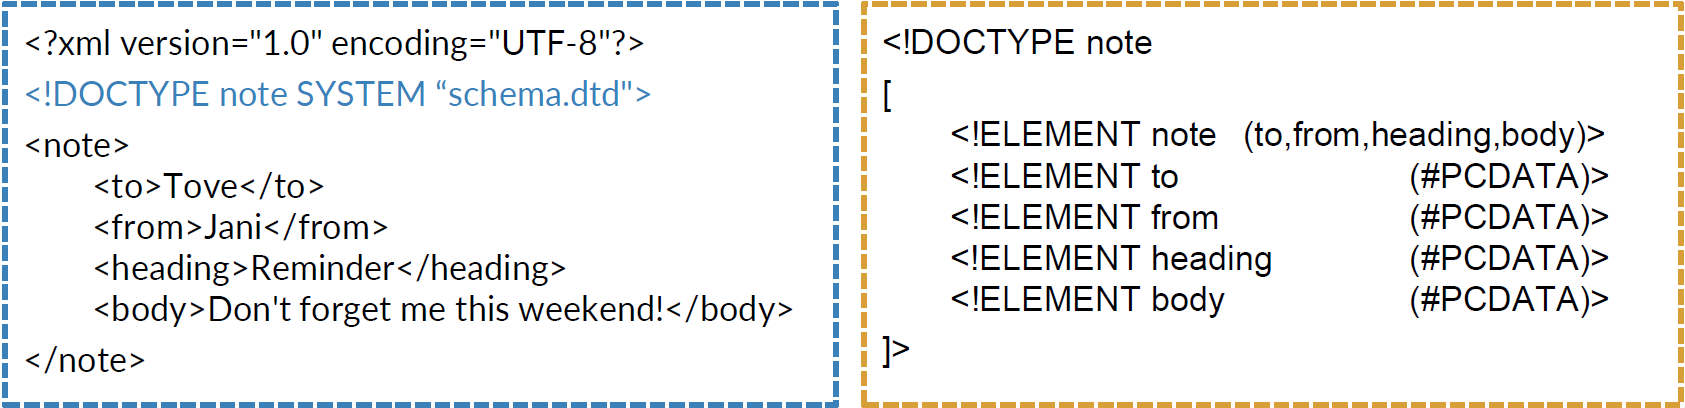
\includegraphics[width=\textwidth]{Images/DTD_validation_example.png}
  \caption{Example of validation using DTD}
\end{figure}

A DTD can be embedded directly within an XML document or linked as an external file using a \texttt{<!DOCTYPE>} declaration. This declaration appears after the optional XML prolog but before the root element and specifies the name of the root element that the DTD defines. \\

To define the structure of elements, DTD uses the \texttt{<!ELEMENT>} directive. This declaration specifies the element's name and its content model, which dictates what the element is allowed to contain. The primary content models include \texttt{EMPTY}, \texttt{ANY}, element content (sequences of child elements), and mixed content (\texttt{\#PCDATA} combined with child elements, PCDATA stands for Parsed Character Data). The occurrence of child elements can be controlled with modifiers: \texttt{?} for zero or one, \texttt{*} for zero or more, and \texttt{+} for one or more. \\

To define attributes, DTD uses the \texttt{<!ATTLIST>} directive. Each attribute definition consists of three parts: the attribute name, its type, and a default value declaration.

\begin{itemize}
    \item
    \textbf{Attribute Types} in DTD are limited but provide basic constraints:
    \begin{itemize}
        \item 
        \texttt{CDATA}: Character data (a simple string).

        \item 
        \textbf{Enumerated List:} A predefined list of acceptable values, such as \texttt{(left|center|right)}.

        \item 
        \texttt{ID}: A unique identifier for the element within the document.

        \item 
        \texttt{IDREF / IDREFS}: A reference (or list of references) to an element with a corresponding \texttt{ID}.

        \item 
        \texttt{ENTITY}: A shortcut to a special character or string.
    \end{itemize}

    \item 
    \textbf{Default Value Declarations} specify an attribute's behavior:
    \begin{itemize}
        \item \textbf{Optional Attributes:}
        \begin{itemize}
            \item \texttt{\#IMPLIED}: The attribute is optional and has no default value.

            \item \texttt{"default value"}: The attribute is optional; if omitted, the specified default value is used.
        \end{itemize}

        \item \textbf{Mandatory Attributes:}
        \begin{itemize}
            \item \texttt{\#REQUIRED}: The attribute must be present, and no default value is provided by the schema.

            \item \texttt{\#FIXED "value"}: The attribute must be present and must have the specified fixed value.
        \end{itemize}
    \end{itemize}
\end{itemize}

Despite its utility, DTD has significant limitations. For instance, while a DTD can enforce an enumerated list of values for an attribute, it cannot enforce a similar constraint on the text content of an element. This seemingly minor limitation has profound consequences. It meant that while metadata in an attribute could be tightly controlled, the core content of an element could not be validated against a specific business vocabulary without custom application code, undermining the goal of robust, schema-driven data interchange. This deficiency was a primary catalyst for the creation of XSD.

\section{XML Schema Definition (XSD)}

\begin{figure}
  \centering
  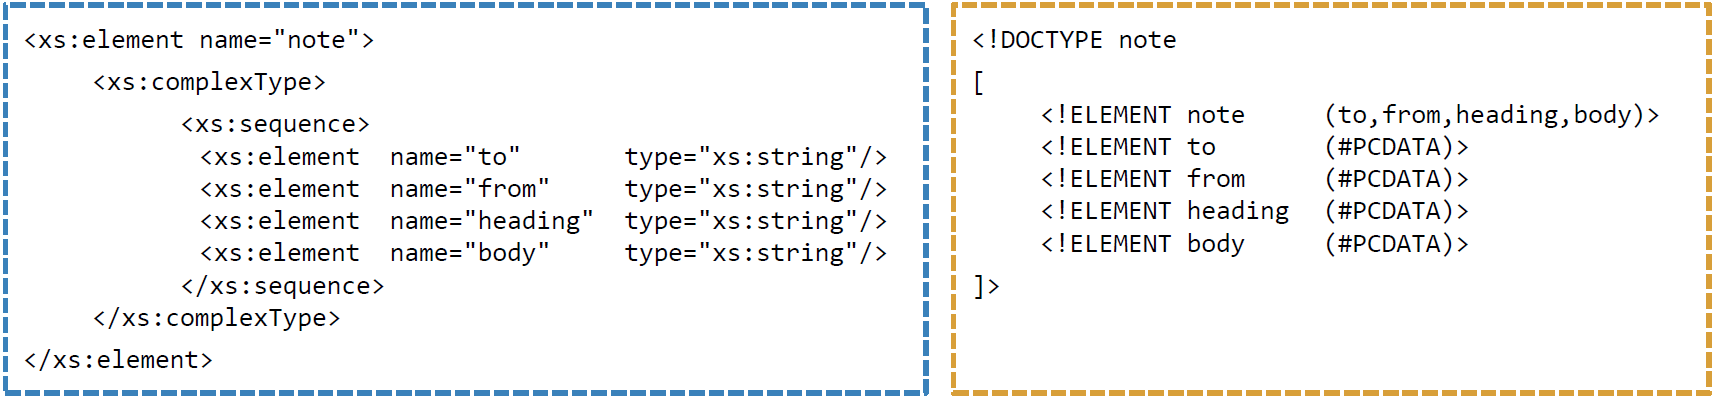
\includegraphics[width=\textwidth]{Images/XSD_validation_example.png}
  \caption{Comparison between XSD validation and DTD validation}
\end{figure}

\begin{table}
    \centering
    \begin{tabular}{|c|c|c|} \hline
        \textbf{Feature} & \textbf{DTD} & \textbf{XSD} \\ \hline

        Syntax & Own format & XML \\ \hline

        Notation & Compact & Verbose \\ \hline

        Data type & Simple (PCDATA, CDATA) & Advanced \\ \hline

        Namespace & Not supported & Supported \\ \hline
    \end{tabular}
    \caption{DTD and XSD feature comparison}
\end{table}

\begin{figure}
  \centering
  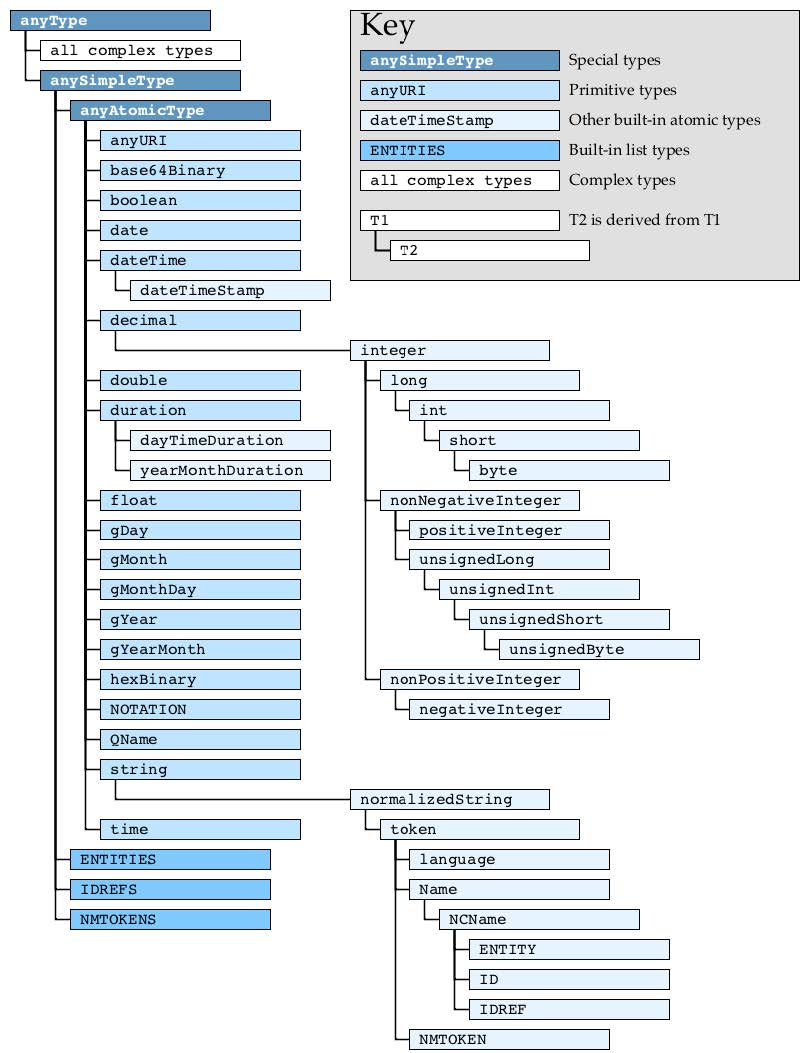
\includegraphics[width=\textwidth]{Images/XML_schema.jpg}
  \caption{XML Schema}
\end{figure}

XML Schema Definition (XSD) was developed by the W3C as a more powerful and flexible alternative to DTD. Its key advantages are that it is written in XML syntax, fully supports namespaces, and provides a rich and extensible system of data types. This allows for much more precise and granular validation of XML documents and makes the conversion of the data between different data types possible. The XSD specification itself is divided into two main parts: \textit{Part 1: Structures}, which defines how to describe the hierarchy and content models of elements, and \textit{Part 2: Datatypes}, which provides a comprehensive library of built-in types. \\

An XSD document, also known as a schema, has \texttt{<xs:schema>} as its root element. This element typically defines namespaces, including the \texttt{targetNamespace}, which specifies the unique URI for the vocabulary being defined. An XML document references its corresponding schema using the \texttt{xsi:schemaLocation} attribute, which points to the location of the XSD file.

\subsection{Simple Types and Restrictions (Facets)}

In XSD, simple elements and attributes—those containing only text and no child elements or attributes—are defined using the \texttt{<xs:element>} and \texttt{<xs:attribute>} declarations. Each declaration includes a name and a \texttt{type}, which can be one of the many built-in datatypes like \texttt{xs:string}, \texttt{xs:integer}, \texttt{xs:date}, or \texttt{xs:boolean}. \\

This rich type system is a major advantage over DTD. Furthermore, XSD allows these types to be constrained using restrictions, also known as \textbf{facets}. Facets define rules that the data must conform to, enabling highly specific validation. Key facets include:

\begin{itemize}
    \item
    \texttt{enumeration}: Defines a list of acceptable values for a type.

    \item 
    \texttt{minInclusive} / \texttt{maxInclusive}: Specifies the minimum and maximum acceptable numeric values.

    \item 
    \texttt{length} / \texttt{minLength} / \texttt{maxLength}: Constrains the number of characters in a string.

    \item 
    \texttt{pattern}: Defines a regular expression that the value must match.

    \item 
    \texttt{totalDigits}: Specifies the exact number of digits allowed in a number.
\end{itemize}

\subsection{Complex Types}

A \textbf{complex type} is a type definition for an element that can contain child elements and/or have attributes. These types can be defined 'anonymously' inside an element declaration for one-time use, or they can be given a unique name, allowing them to be defined once and reused for multiple elements and attributes throughout the schema. XSD defines four kinds of complex types, providing patterns for all common structural needs:

\begin{enumerate}
    \item
    \textbf{Empty Elements:} These elements have no text or child elements but are allowed to have attributes.

    \item 
    \textbf{Elements-Only Content:} These elements contain only other child elements, with no intermingled text. This is common for structured data records.

    \item 
    \textbf{Text-Only Content (Simple Content):} These elements contain only text but may also have attributes. This allows for simple values to be annotated with metadata.

    \item 
    \textbf{Mixed Content:} These elements can contain a combination of text and child elements. This is enabled by setting the \texttt{mixed="true"} attribute on the complex type definition and is useful for document-centric XML.
\end{enumerate}

\subsection{Indicators for Controlling Structure}

Within a complex type, indicators are used to define the order, choice, and occurrence of child elements, giving schema authors precise control over the document structure. \\

First, \textbf{Order Indicators} define the relationships between sibling elements:

\begin{itemize}
    \item 
    \texttt{<xs:all>}: All of the specified children elements must appear, but they can be in any order.

    \item 
    \texttt{<xs:choice>}: Only one of the specified children elements can occur.
    
    \item 
    \texttt{<xs:sequence>}: Children elements must appear in the exact order specified in the schema.
\end{itemize}

Second, \textbf{Occurrence Indicators} control how many times an element can appear:

\begin{itemize}
    \item
    \texttt{minOccurs}: Specifies the minimum number of times an element can occur. The default is \texttt{1}.

    \item 
    \texttt{maxOccurs}: Specifies the maximum number of times an element can occur. The default is \texttt{1}. It can also be set to \texttt{unbounded} to allow for an unlimited number of occurrences.
\end{itemize}

Third, \textbf{Group Indicators} are useful to create groups of related elements or attributes. This conveniently allows us to refer to them using a single line of code.

\begin{itemize}
    \item 
    \texttt{group (Element group)}: Defines a group of related elements.

    \item 
    \texttt{attributeGroup}: Defines a group of related attributes.
\end{itemize}

Once a document's structure is guaranteed through validation, the focus shifts from definition to interaction. The broader XML ecosystem provides a suite of powerful languages for querying, transforming, and ultimately leveraging the data contained within.

\begin{lstlisting}[language=XML, caption=Example of elements group definition - Courtesy of tutorialspoint.com]
    <xs:group name = "infogroup">
       <xs:sequence>
          <xs:element name = "firstname" type = "xs:string"/>
          <xs:element name = "lastname" type = "xs:string"/>
          <xs:element name = "birthdate" type = "xs:date"/>
       </xs:sequence>
    </xs:group>
    
    <xs:element name = "student" type = "studentType"/>
    
    <xs:complexType name = "studentType">
       <xs:sequence>
          <xs:group ref = "infogroup"/>
          <xs:element name = "marks" type = "xs:integer"/>
       </xs:sequence>
    </xs:complexType>
\end{lstlisting}

\begin{lstlisting}[language=XML, caption=Example of attributes group definition - Courtesy of tutorialspoint.com]
    <xs:attributeGroup name = "infogroup">
       <xs:sequence>
          <xs:attribute name = "firstname" type = "xs:string"/>
          <xs:attribute name = "lastname" type = "xs:string"/>
          <xs:attribute name = "birthdate" type = "xs:date"/>
       </xs:sequence>
    </xs:attributeGroup>
    
    <xs:element name = "student" type = "studentType"/>
    
    <xs:complexType name = "studentType">
       <xs:sequence>
          <xs:attributeGroup ref = "infogroup"/>
          <xs:element name = "marks" type = "xs:integer"/>
       </xs:sequence>
    </xs:complexType>
\end{lstlisting}

\chapter{The Broader XML Ecosystem}

Beyond defining and validating XML's structure, a family of W3C-specified languages exists to query, transform, and manipulate XML documents. These technologies work together to form a powerful ecosystem for processing XML data.

\begin{itemize}
    \item
    \textbf{XPath (XML Path Language):} This is a language for addressing and selecting nodes within an XML document's tree structure. Using path-like expressions, XPath allows you to navigate through elements and attributes to pinpoint specific pieces of data. It is not a standalone language but a foundational component used by both XSLT and XQuery.

    \item 
    \textbf{XQuery (XML Query Language):} This is a language for finding and extracting information from one or more XML documents. Functionally, it is to XML what SQL is to relational databases. It uses XPath expressions to query collections of XML data and can return results as new XML documents.

    \item 
    \textbf{XSLT (eXtensible Stylesheet Language Transformations):} This is a declarative language that leverages the latter two to transform an XML document into another format. Common transformations include converting an XML document into a different XML structure, an HTML web page, or a plain text file.
\end{itemize}

The principles of XML—its strict syntax and structured nature—have been applied to many domains, with one of the most notable being the attempt to reformulate HTML itself.

\chapter{Case Study: The Rise and Fall of XHTML}

XHTML stands as a significant historical case study on the application of XML's rigorous principles to the world of web pages. \textbf{XHTML (eXtensible HyperText Markup Language)} was a reformulation of HTML 4.01 designed to conform to the strict syntax of XML. Its primary motivation was to create a cleaner, more well-defined, and reliably parsable markup language for an expanding ecosystem of web-enabled devices, such as mobile phones, that lacked the processing power to handle the lenient parsing required by traditional HTML. \\

The critical rule that ultimately led to its failure in widespread adoption was a direct consequence of its XML heritage: an XHTML document, like any XML application, had to be \textbf{well-formed}. If a document contained even a minor syntax error—such as an unclosed tag—an XHTML-compliant browser was instructed not to render the page at all. Instead, it was required to halt processing and display a syntax error message to the user. This new standard, developed in parallel with the XML 1.1 specification which was tuned to support it, represented a philosophically pure but practically unworkable approach to web markup. \\

This behavior stood in stark contrast to that of standard HTML browsers, which were historically designed to be lenient. HTML browsers would make a best-effort attempt to render malformed pages, forgiving common errors to ensure that the content was still visible to the user. \\

The practical implication of this difference was profound. By the time XHTML was introduced, the vast majority of existing web pages—and a large number of newly created ones—contained syntax errors. Enforcing the strict XHTML rule would have meant that most of the web would simply fail to display. Web users, who cared about content rather than syntactic purity, would be faced with error messages instead of websites. This made the standard unworkable in practice. The approach was ultimately abandoned, and the web development community moved toward HTML5, which embraced a more pragmatic, fault-tolerant parsing model. \\

The story of XHTML serves as a powerful lesson on the inherent tension between the pursuit of rigorous technical standards and the practical realities of a large-scale, decentralized, and imperfectly implemented ecosystem.

\end{document}
